\subsubsection{Environment}

\begin{figure}[H]
\centering
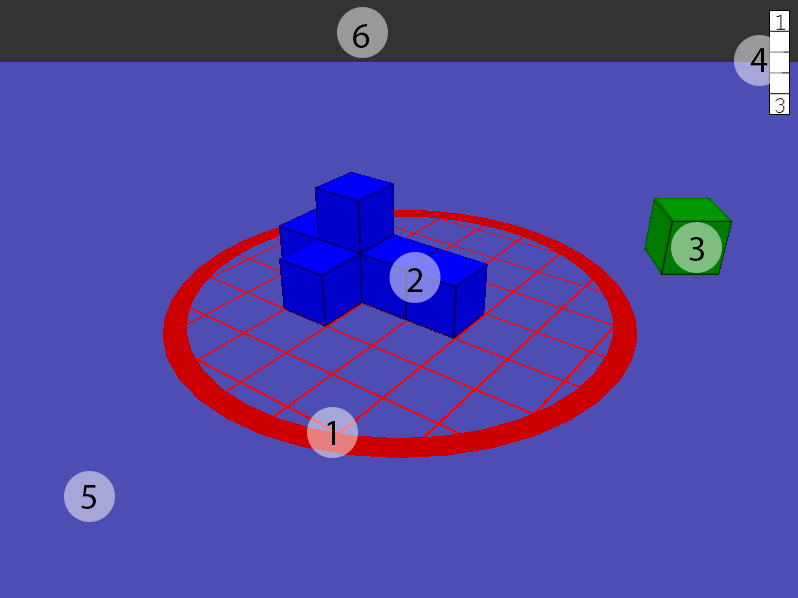
\includegraphics[width=\textwidth]{env_comps}
\caption{\label{fig:environmentcomps} Common rendering of the task environment. Visual elements: 1-Circular~grid 2-Building~blocks 3-Creation~block 4-Target~indicator 5-Floor 6-Horizon}
\end{figure}

\noindent The task environment is a virtual graphical computer program for building virtual block structures using either a Leap Motion or keyboard and mouse. Figure~\ref{fig:environmentcomps} shows a common rendering from the task environment in which all visual elements have been labeled. In the center of the screen users are presented with a circular grid that is segmented into several squares, effectively representing a grid with an circular border. On this grid building blocks can be positioned, either directly on the grid or stacked on top of other building blocks. New building blocks can be obtained by interacting (clicking with the mouse or grabbing with the Leap Motion) with the creation block just next to the circular grid. The target indicator on the top right corner gives the user a representation of the block structure that should be created on the grid before the user can move further.

\paragraph{Circular grid}
The circular grid is made out of square grid-cells and a limit circle which has a radius that is slightly bigger than $3.5$ grid-cells width. The grid is able to rotate $360^{\circ}$ around the y-axis of the center of this grid (the origin). In resting state the grid and limit circle have a red color, but while the circle is rotated by the user the limit circle temporarily becomes orange until it reaches resting state once more. 

\paragraph{Building blocks}
The building blocks are 3D cubes with dimensions corresponding to $1\times 1\times 1$ the width of a grid-cell and all have black outline at the edges. Building blocks can be lifted, dragged around, and dropped by the user. While building blocks are lifted they cast a shadow directly below them in order to know their position relative to the grid. In resting state the building blocks are blue, when they are being dragged they are orange and when a user points at them and does not drag anything they become light-blue. 

\paragraph{Creation block}
The creation block has the same dimensions as the building blocks, but has a different color. A user can use the creation block to obtain new building blocks by interacting with it. When a user points at the creation block it turns light-green, otherwise it has a dark-green color. In the version of the environment used for the experiment the creation block was positioned one grid-cell width above the floor level to compensate for the limited vertical detection range of the LEAP Motion.

\paragraph{Target indicator}
The target indicator is a 2D image always visible to the user. It shows the currently active target structure (or goal) that should be created by the user with the building blocks in order to advance to the next task and to complete the experiment. The image is always shown in a single orientation, but actual task completion can be achieved by creating a $90^{\circ}$, $180^{\circ}$ or $270^{\circ}$ degree rotated version of the target structure within the grid as well. Also it does not matter where in the grid the solution is created.

\paragraph{Floor}
The floor is merely a plane that indicates the lower limit of where building blocks can be positioned. It also serves as a surface to show the shadows from the building blocks on.

\paragraph{Horizon}
A small strip of horizon is made visible to help the user understand the orientation when tilting the camera up and down. The current color of the horizon is dark-gray.


\paragraph{Ghost block}
The ghost block is a special transparent-red block that has the same size as a normal building block. It only appears when a building block is dragged but gets stuck behind other blocks. Such a situation is depicted in Figure~\ref{fig:ghostblock}. This ghost block helps the user to realize that an illegal dragging operation is being performed and what the current 3D location of the dragged building block would be if it would not have been stuck.

\begin{figure}[H]
\centering
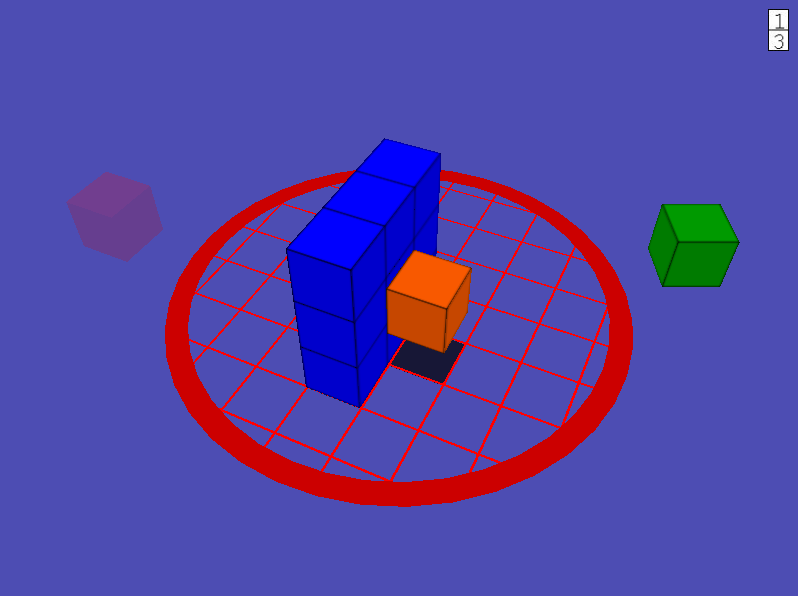
\includegraphics[width=0.5\textwidth ]{ghost_block}
\caption{\label{fig:ghostblock} The ghost block appears when a block gets stuck behind other blocks while dragging. In this case the user was dragging a building block from right to left, but it got stuck behind a wall of other building blocks.}
\end{figure}


\paragraph{LEAP Motion hand}



\paragraph{Color and lighting settings}

All the previously described components have one or more color states associated with them, depending on the state of the respective component and are listed in Table~\ref{tab:colors}. Each  color state consist out of a red (r), green (g), blue (b) and an alpha (a) component contributing to the color intensity and can optionally have a thin black border (outline) at the edges of the objects. Also all visual components, except the horizon, are influenced by two types of virtual lighting: 
\begin{enumerate}
	\item{\textbf{Ambient lighting:}} All color intensities are multiplied by $0.8$ on default.
	\item{\textbf{Parallel directional light:}} All the color intensities of non-transparent object surfaces perpendicular to the y-axis are restored to their original color values.
\end{enumerate}


\begin{table}[H]
\centering
\begin{tabular}{|c|c|c|c|c|c|c|c|}
\hline
\textbf{object} & \textbf{state} & \textbf{r} & \textbf{g} & \textbf{b} & \textbf{a} & \textbf{outline} & \textbf{common name}\\ \hline\hline
Building block & resting & 0 & 0 & 255 & 255 & x & blue \\ 
 & dragged & 255 & 191 & 0 & 255 & x & orange \\ 
 & pointed & 138 & 149 & 255 & 255 & x & light-blue \\ \hline 
Creation block & resting & 0 & 178 & 0 & 255 & x & dark-green \\ 
 & pointed & 158 & 255 & 149 & 255 & x & light-green\\ \hline 
Ghost block & - & 255 & 0 & 0 & 51 & & transparent-red \\ \hline
LEAP Motion hand & - & 0 & 255 & 0 & 77 & & transparent-green  \\ \hline 
Grid & resting & 255 & 0 & 0 & 255 & & red \\ 
 & rotating & 255 & 191 & 0 & 255 & & orange \\ \hline 
Floor & - & 77 & 77 & 179 & 255 & & purple/blue \\ \hline 
Horizon & - & 51 & 51 & 51 & 255 & & dark-gray \\ \hline 
\end{tabular}
\caption{\label{tab:colors} Color states of the objects within the task environment.}
\end{table}

\paragraph{Design rationale}
The program was developed with the use of jMonkeyEngine, an open source 3D game engine written in Java. For development we used the Software Development Kit that comes with the engine, which provides a high level interface for numerous 3D functions and data-structures (e.g. spatial manipulation, quaternions and 3D meshes) and also provides a high degree of control for developers by being completely compatible with the Java programming language. 

Both the User Interface (UI) and the user interactions were designed to be minimalistic, simple and intuitive in order to prevent users having to learn a lot before they could use the system. 
